\documentclass{beamer}
\usetheme[hideothersubsections]{Berkeley}
\usepackage{tikz}
\usetikzlibrary{fadings}
\usetikzlibrary{positioning}
\usepackage{listings}
\usepackage{array}
\usepackage[export]{adjustbox}
\newcolumntype{L}{>{\centering\arraybackslash}m{3cm}}
\makeatletter
\setbeamertemplate{sidebar \beamer@sidebarside}%{sidebar theme}
  {
    \beamer@tempdim=\beamer@sidebarwidth%
    \advance\beamer@tempdim by -6pt%
    \insertverticalnavigation{\beamer@sidebarwidth}%
    \vfill
    \ifx\beamer@sidebarside\beamer@lefttext%
    \else%
      \usebeamercolor{normal text}%
      \llap{\usebeamertemplate***{navigation symbols}\hskip0.1cm}%
      \vskip2pt%
    \fi%
  }%
\makeatother


\title{Automatic Detection of Pseudo-Tested Methods in a Test Suite Using Fault Injection}
\author{Nicholas Tocci}
\date{\today}

\begin{document}
%%%%%%%%%%%% Introduction %%%%%%%%%%%%%%%%%%%%%%%%%%%%%%%%%%%%%%%%%%%%%%%%%%%
\section{Introduction}
\begin{frame}
	\frametitle{Introduction}
	\titlepage
\end{frame}
%%%%%%%%%%%% Problem %%%%%%%%%%%%%%%%%%%%%%%%%%%%%%%%%%%%%%%%%%%%%%%%%%%
\section{Problem}
\label{sec:problem}
%%%%%%%%%%%% Slide %%%%%%%%%%%%%%%%%%%%%%%%%%%%%%%%%%%%%%%%%%%%%%%%%%%
\begin{frame}
	\frametitle{Problem}
	\begin{center}
		\huge{How can we know if our test suites are effective?}

		
\includegraphics[scale = .25]{images/thumb}
	\end{center}
\end{frame}

% Beginning of Current Metrics
\subsection{Coverage}
%%%%%%%%%%%% Slide %%%%%%%%%%%%%%%%%%%%%%%%%%%%%%%%%%%%%%%%%%%%%%%%%%%
\begin{frame}
	\frametitle{Coverage}
		\begin{center}
			\huge{Coverage}

			
\includegraphics[scale = 0.25]{images/percent.png}

			\textbf{\textit{Def}}: \% of a system that has been tested.
		\end{center}




\end{frame}

\subsubsection{Calculation}
%
% This sections will explain why Passing Test Cases do not indicate a good Test Suite.
%
\begin{frame}
	\frametitle{Calculation}
	\begin{center}
		\begin{equation*}
			Function Coverage = \frac{Number of Tested Methods}{Total Number of Methods}
		\end{equation*}
	\end{center}
\end{frame}

\subsubsection{Coverage vs Adequate Coverage}
%
% This sections will explain why High Coverage can mislead a developer.
%
\begin{frame}
	\frametitle{High Coverage}
		\begin{center}
			
\includegraphics[scale = .15]{images/percentEquals}
		\end{center}
\end{frame}


\section{Pseudo-tested Methods}
\label{sec:pseudo-tested methods}
\begin{frame}
	\frametitle{Pseudo-tested Methods}
	\begin{center}
    \huge{Pseudo-tested Methods}
  \end{center}
\end{frame}

\subsection{Defintion}
\begin{frame}
  \frametitle{Definition}
    \begin{center}
      \textbf{What is a Pseudo-tested Method?}

      \vspace{10mm}
      
\includegraphics{images/passing}

      \vspace{10mm}
      \textbf{\textit{Def}}: It will never fail.
    \end{center}
\end{frame}

\subsection{Detection}
\begin{frame}
  \frametitle{Detection}
    \begin{center}
      \textbf{How Can We Detect Pseudo-tested Methods}

			\vspace{20mm}
			\textbf{It is harder than you think!}

    \end{center}
\end{frame}

\begin{frame}[fragile]
\frametitle{Example of a Pseudo-tested method}
	\begin{figure}[t!, scale = .75]
	\begin{lstlisting}[language = Python, basicstyle=\small, backgroundcolor = \color{lightgray}]
numbers.py:
def numberOrder(n):
  numbersSorted = sorted(n)
  return numbersSorted


test_numbers.py:
def test_numbers_ordered():
  numbers = set([2,4,3,1])
  sortedNumbers = set([1,2,3,4])
  orderedNumbers = numberOrder(numbers)
  assert numbers == sortedNumbers
	\end{lstlisting}
	\end{figure}
\end{frame}


\section{Function-Fiasco}
\label{sec:function-fiasco}
\subsection{What is Function-Fiasco}
\begin{frame}
  \frametitle{What is Function-Fiasco}
    \begin{center}
      \huge{\textbf{A Pseudo-tested method detection tool}}

      
\includegraphics[scale = .15]{images/wrench}
    \end{center}
\end{frame}

\begin{frame}[fragile]
  \frametitle{Decorator Function}
  \begin{figure}[t!, scale = .75]
	\begin{lstlisting}[language = Python, basicstyle=\tiny, backgroundcolor = \color{lightgray}]
  def skipper(func):
      functionsComplete = globs.functionsComplete
      checked = checkFunctionsComplete(func, functionsComplete)
      globs.checked = str(checked)
      if checked == True and globs.firstExe == True:
          def wrapper(*args, **kwargs):
              checkType(var, func.__name__)
              return var
          return wrapper
      elif checked == True and globs.firstExe == False:
          def doFunc(*args, **kwargs):
              var = func(*args, **kwargs)
              return checkType(var, func.__name__)
          return doFunc
      else:
          def doFunc(*args, **kwargs):
              var = func(*args, **kwargs)
              return var
          return doFunc
  \end{lstlisting}
\end{figure}
\end{frame}

\begin{frame}
  \frametitle{Execution Flow}
  \begin{center}
    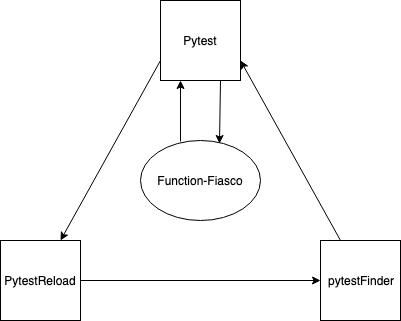
\includegraphics[scale = .5]{images/pytestFlow.png}
  \end{center}
\end{frame}

\subsection{Flow}
\begin{frame}
  \frametitle{Flow to system}
    \begin{center}
      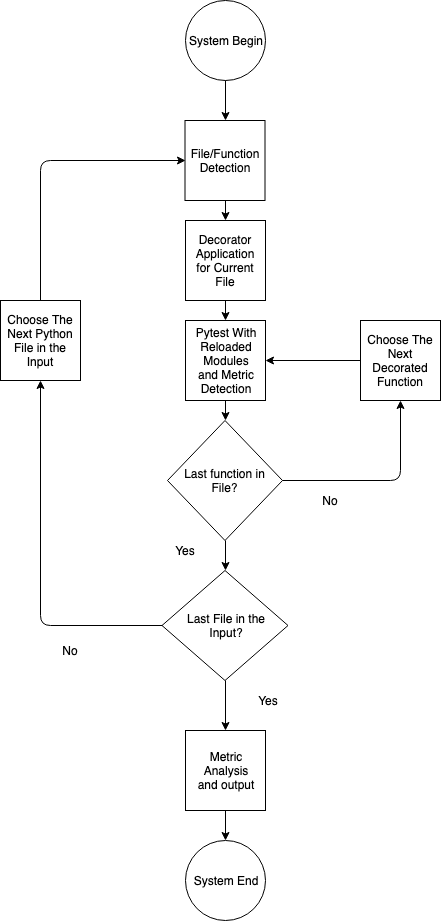
\includegraphics[scale = .22]{images/flow.png}
    \end{center}
\end{frame}


\section{Evaluation Strategy}
\label{sec:Evaluation Strategy}
\subsection{Coverage Calculation}
\begin{frame}
\frametitle{Coverage Calculation}
\begin{center}
  \begin{equation*}
    FunctionCoverage = \frac{Number of Tested Methods}{Total Number of Methods}
  \end{equation*}
\end{center}
\end{frame}

\begin{frame}
  \frametitle{Coverage Example}
  \begin{center}

  \begin{table}[htbp]
  %   \centering
   \resizebox{6.5cm}{!}{%
    \begin{tabular}{|c|c|c|c|c|c|}
      \hline
  %
      \bf NUMM     & \bf NUMTM & \bf Function Coverage \\ \hline\hline
      40  & 25  & 62.5\%  \\ \hline
  %
  %
    \end{tabular}%
    }

  \end{table}

  \end{center}
\end{frame}

\subsection{Truly-Tested-Method Calculation}
\begin{frame}
  \frametitle{Truly-Tested-Method Calculation}
  \begin{itemize}
    \item \textbf{Number of Truly-Tested-Methods = NUMTTM}

    \item \textbf{Number of Tested Methods = NUMTM}

    \item \textbf{Number of Pseudo-tested Methods = NUMPTM}
  \end{itemize}

  \begin{center}
    \begin{equation*}
      NUMTTM = NUMTM - NUMPTM
    \end{equation*}
  \end{center}
\end{frame}

\begin{frame}
  \frametitle{Truly-Tested-Method Example}
  \begin{center}

  \begin{table}[htbp]
  %   \centering
   \resizebox{6.5cm}{!}{%
    \begin{tabular}{|c|c|c|c|c|c|}
      \hline
  %
      \bf NUMTM     & \bf NUMPTM & \bf NUMTTM \\ \hline\hline
      25  & 3  & 22  \\ \hline
  %
  %
    \end{tabular}%
    }

  \end{table}

  \end{center}
\end{frame}

\begin{frame}
\frametitle{Adequate-Coverage Calculation}
\begin{center}
  \begin{equation*}
    AC = \frac{Number of TrulyTested Methods}{Total Number of Methods}
  \end{equation*}
\end{center}
\end{frame}

\subsection{Metrics Produced}
\begin{frame}
  \frametitle{Output}

    \begin{figure}
    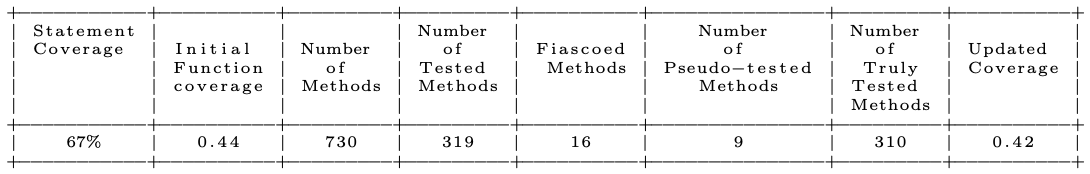
\includegraphics[scale = .55]{images/tableOutput}
    \end{figure}
\end{frame}


\section{Results}
\label{sec:Results}
\begin{frame}
  \frametitle{List of Systems}
  % latex table generated in R 3.4.4 by xtable 1.8-3 package
% Sat Mar 30 16:19:07 2019
\begin{table}[H]
\centering
\begin{tabular}{rlrrr}
  \hline
 & System\_Name & Num\_Methods & Fiascoed & Num\_Tests \\
  \hline
1 & Hashids-Python &  16 &  10 &  59 \\
  2 & Bleach & 368 &   8 & 312 \\
  3 & Pycco &  22 &   6 &  17 \\
  4 & Howdoi &  20 &   2 &  18 \\
  5 & Flashtext &  42 &   7 &  23 \\
  6 & Honcho &  58 &   7 & 124 \\
  7 & Maya &  88 &  13 & 277 \\
  8 & Gator &  91 &  53 & 505 \\
  9 & Hatch & 134 &  14 & 339 \\
  10 & Nikola & 732 &  16 & 205 \\
   \hline
\end{tabular}
\caption{List of systems used for testing.}~\label{sysList}
\end{table}

\end{frame}

\begin{frame}
  \frametitle{Statement Coverage}
  \begin{figure}
  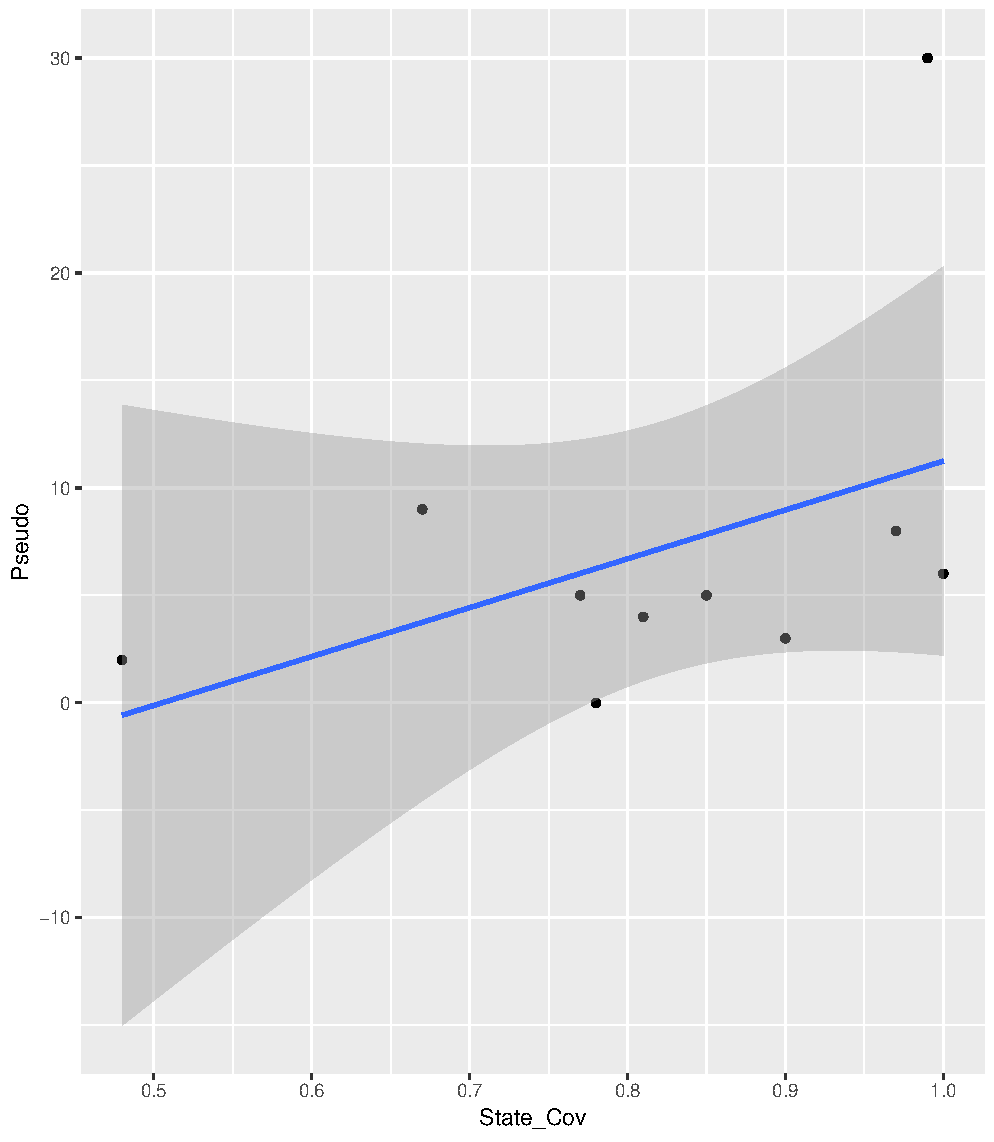
\includegraphics[scale = .35]{images/stateCovPlot}
  \end{figure}
\end{frame}

\begin{frame}
  \frametitle{Type Risk}
  % latex table generated in R 3.5.3 by xtable 1.8-3 package
% Tue Apr  2 04:08:23 2019
\begin{table}[H]
\centering
\begin{tabular}{rlrrl}
  \hline
 & Type & Used & Found & ratio \\
  \hline
1 & Strings &  69 &  33 & 47.8\% \\
  2 & Booleans &  49 &  35 & 73.5\% \\
  3 & Ints &  18 &   4 & 22.2\% \\
  4 & Floats &   1 &   0 & 0\% \\
   \hline
\end{tabular}
\caption{Breakdown of the number of pseudo-tested method per type.}~\label{retTable}
\end{table}

\end{frame}


\section{Conclusion}
\label{sec:Conclusion}

\begin{frame}
  \frametitle{Field Connects}
  \begin{itemize}
    \item {Computer Science}
  \end{itemize}
\end{frame}

\begin{frame}
  \frametitle{Field Connects}
  \begin{itemize}
    \item {Computer Science}
    \item {Software Engineering}
  \end{itemize}
\end{frame}

\begin{frame}
  \frametitle{Field Connects}
  \begin{itemize}
    \item {Computer Science}
    \item {Software Engineering}
    \item {Software Testing}
  \end{itemize}
\end{frame}

\subsection{Impact}
\begin{frame}
  \frametitle{What is the impact of this research?}
  \begin{center}
  %
    \begin{table}[htbp]
      \centering
    \resizebox{9.5cm}{!}{%
      \begin{tabular}{L L L}

  %
        
\includegraphics[scale= 0.1]{images/percent}     & 
\includegraphics[scale = .10]{images/pseudoCheck} & 
\includegraphics[scale = .1]{images/wrench} \\
        Coverage with fault detection  & Better Understanding of Pseudo-tested Methods  & Automatic Detection Tool  \\

  %
      \end{tabular}%
    }
    \end{table}
  \end{center}
\end{frame}

\subsection{Future Research}
\begin{frame}
  \frametitle{Future Research}
  \begin{center}
    \begin{itemize}
      \item {Different Types and Paramaterization}
      \item {Bug Fixes}
      \item {Documentation}
      \item {Further Testing}
    \end{itemize}
    
\includegraphics[scale = 0.25]{images/clock}
  \end{center}
\end{frame}

\subsection{Demo}
\begin{frame}
  \frametitle{Demo}
  \begin{center}
    \large{\textbf{Function-Fiasco}}



    \vspace{10mm}
    \small{Automatic Detection System for Pseudo-tested Methods}
  \end{center}
\end{frame}

\end{document}
